\documentclass{xtikzfig}
  \usetikzlibrary{arrows}
  
\def\tmax{9}
\def\Tmax{2}
\def\Tthr{1.955}
\def\figskip{2.1cm}

\begin{document}
  \begin{tikzpicture}
  
    \node[rotate=90] (T) {Température};

    \node[right of=T, node distance=4.8cm] (B) {
      \begin{tikzpicture}
        %
        \filldraw[fill=gray!50,draw=white] (1,0) rectangle (4,\Tthr); % Nitruration
        %
        %\draw[line width=0.1pt,gray!30,step=10mm] (0,0) grid (\tmax,\Tmax);
        \draw[->,>=latex,very thick] (0,0) -- (0,\Tmax);
        \draw[->,>=latex,very thick] (0,0) -- (\tmax,0);
        %
        \draw[dashed,thick] (0,0) -- (1,\Tthr);
        \draw[thick] (1,\Tthr) -- (4,\Tthr); % Nitruration
        \draw[thick] (4,\Tthr) -- (4.1,0.1); % Trempe
        %
        \node at (2.5,1) {\footnotesize{}Nitruration};
        \draw[->,>=latex,thin] (5,1.5) -- (4.1,1);
        \node at (5,1.6) {\tiny{}Trempe};
        \node at (0.25,1.75) {\footnotesize{}b)};
        \node[rotate=62.9] at (0.6,1.4) {\tiny{}Chauffage};
      \end{tikzpicture}
    };
    
    \node[above of=B, node distance=\figskip] (A) {
      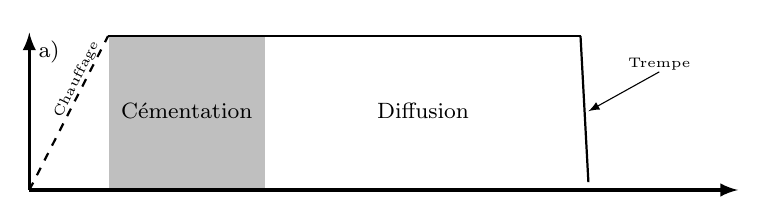
\begin{tikzpicture}
        %
        \filldraw[fill=gray!50,draw=white] (1,0) rectangle (3,\Tthr); % Cementation
        %
        %\draw[line width=0.1pt,gray!30,step=10mm] (0,0) grid (\tmax,\Tmax);
        \draw[->,>=latex,very thick] (0,0) -- (0,\Tmax);
        \draw[->,>=latex,very thick] (0,0) -- (\tmax,0);
        %
        \draw[dashed,thick] (0,0) -- (1,\Tthr);
        \draw[thick] (1,\Tthr) -- (3,\Tthr); % Cementation
        \draw[thick] (3,\Tthr) -- (7,\Tthr); % Diffusion
        \draw[thick] (7,\Tthr) -- (7.1,0.1); % Trempe
        %
        \node at (2,1) {\footnotesize{}Cémentation};
        \node at (5,1) {\footnotesize{}Diffusion};
        \draw[->,>=latex,thin] (8,1.5) -- (7.1,1);
        \node at (8,1.6) {\tiny{}Trempe};
        \node at (0.25,1.75) {\footnotesize{}a)};
        \node[rotate=62.9] at (0.6,1.4) {\tiny{}Chauffage};
      \end{tikzpicture}
    };
  
    \node[below of=B, node distance=\figskip] (C) {
      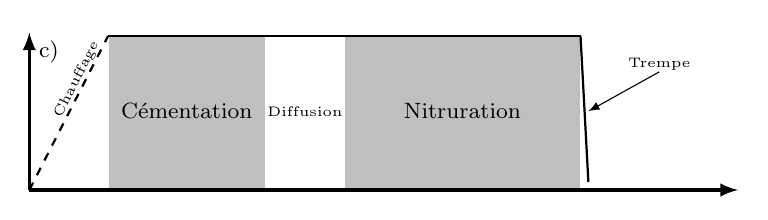
\begin{tikzpicture}
        %
        \filldraw[fill=gray!50,draw=white] (1,0) rectangle (3,\Tthr); % Cementation
        \filldraw[fill=gray!50,draw=white] (4,0) rectangle (7,\Tthr); % Nitruration
        %
        %\draw[line width=0.1pt,gray!30,step=10mm] (0,0) grid (\tmax,\Tmax);
        \draw[->,>=latex,very thick] (0,0) -- (0,\Tmax);
        \draw[->,>=latex,very thick] (0,0) -- (\tmax,0);
        %
        \draw[dashed,thick] (0,0) -- (1,\Tthr);
        \draw[thick] (1,\Tthr) -- (3,\Tthr); % Cementation
        \draw[thick] (3,\Tthr) -- (4,\Tthr); % Diffusion
        \draw[thick] (4,\Tthr) -- (7,\Tthr); % Nitruration
        \draw[thick] (7,\Tthr) -- (7.1,0.1); % Trempe
        %
        \node at (2,1) {\footnotesize{}Cémentation};
        \node at (3.5,1) {\tiny{}Diffusion};
        \node at (5.5,1) {\footnotesize{}Nitruration};
        \draw[->,>=latex,thin] (8,1.5) -- (7.1,1);
        \node at (8,1.6) {\tiny{}Trempe};
        \node at (0.25,1.75) {\footnotesize{}c)};
        \node[rotate=62.9] at (0.6,1.4) {\tiny{}Chauffage};
      \end{tikzpicture}   
    };
  
    \node[below of=C, node distance=1.3cm] (D) {
      
\begin{tikzpicture}       
        \node at (4.5,-0.5) {Temps};
      \end{tikzpicture}
    };
  \end{tikzpicture}
\end{document}